\documentclass[fadttsterUserGuide_master]{subfiles}

\newpage
\begin{document}
	\part{Advanced use of FADTTSter}
	The following sections will help you to use FADTTSter more efficiently with some very useful features.
	
	\section{Configuration files}
	In order to prevent the user from entering the settings in the GUI over and over again, we can use the configuration files. The settings are split into two groups: \textit{Para} and \textit{Soft}. \textit{Soft} rounds up all settings related to the software part while \textit{Para} gathered the rest.
	\vfill
	\begin{figure}[H]
  		\centering
    	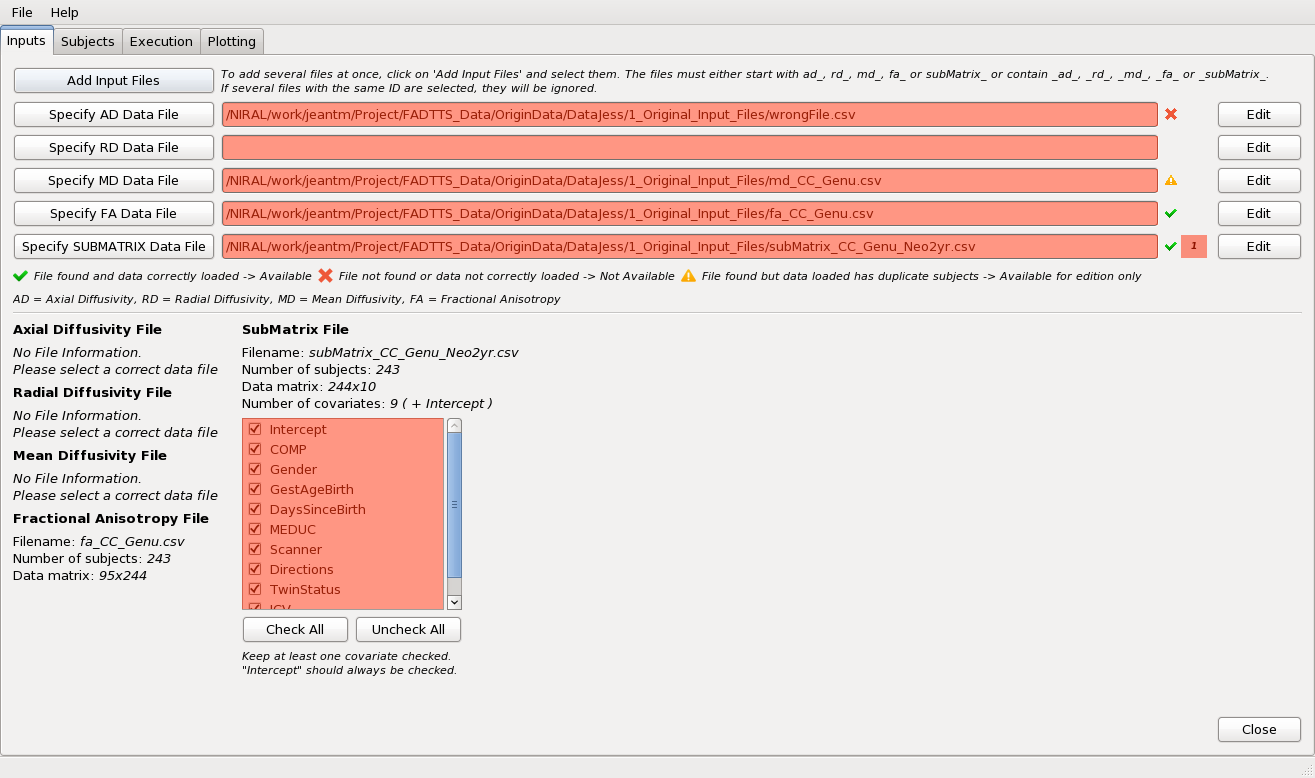
\includegraphics[width=1.0\textwidth]{inputTab_Conf}
    	\caption{\textit{Para} settings (red)}
    	\label{fig:inputTab_Conf}
    \end{figure}
    \vfill
    \newpage
    
    \begin{figure}[H]
  		\centering
    	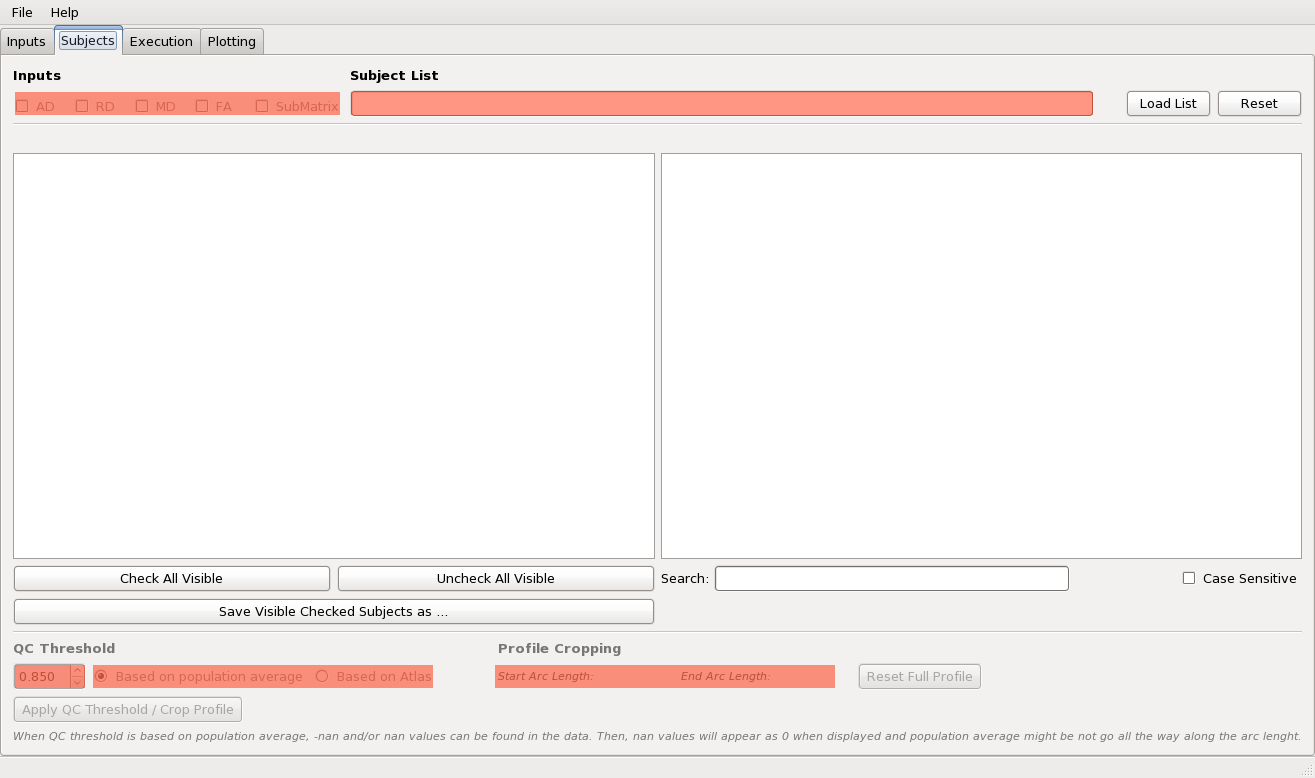
\includegraphics[width=1.0\textwidth]{subjectsTab_Conf}
    	\caption{\textit{Para} settings (red)}
    	\label{fig:subjectsTab_Conf}
    \end{figure}
    \vfill
    \begin{figure}[H]
  		\centering
    	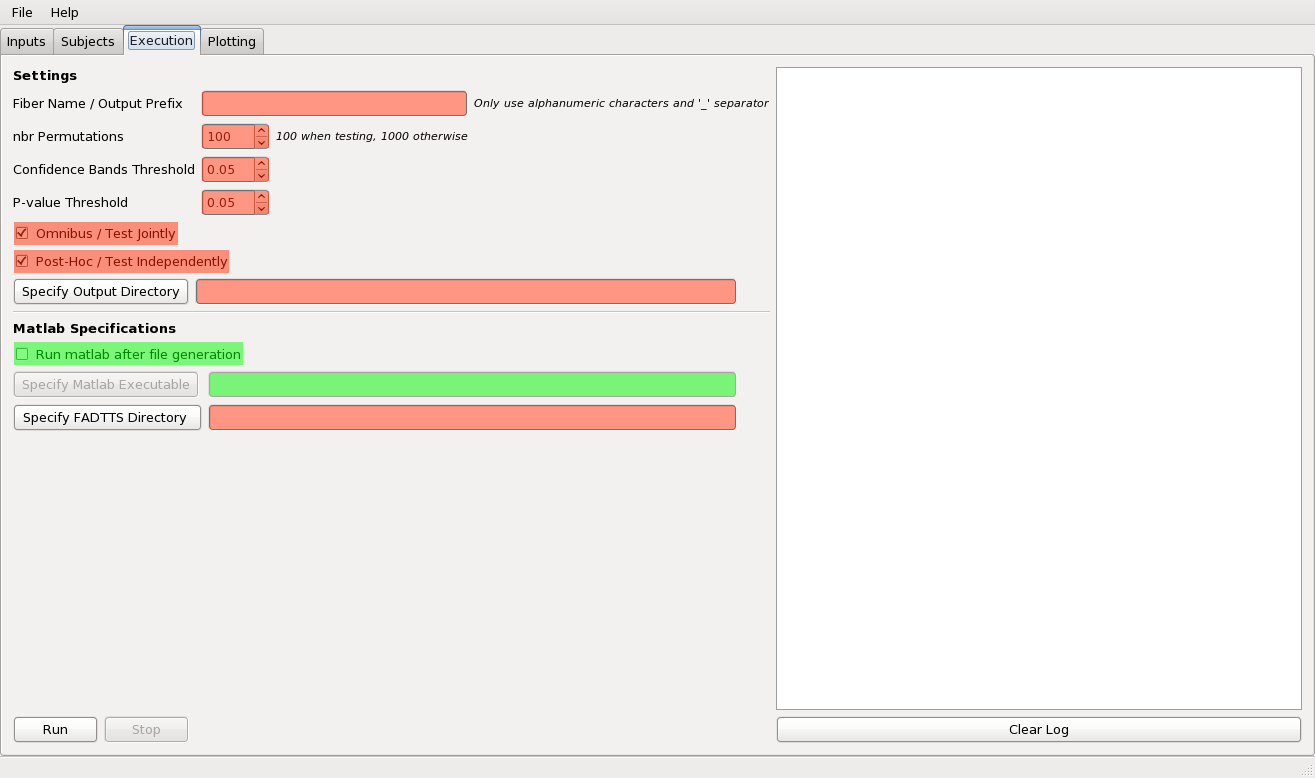
\includegraphics[width=1.0\textwidth]{executionTab_Conf}
    	\caption{\textit{Para} settings (red) and \textit{Soft} settings (green) that can be set with the configuration files}
    	\label{fig:executionTab_Conf}
    \end{figure}
    \vfill
    \newpage
    
    \begin{figure}[H]
  		\centering
    	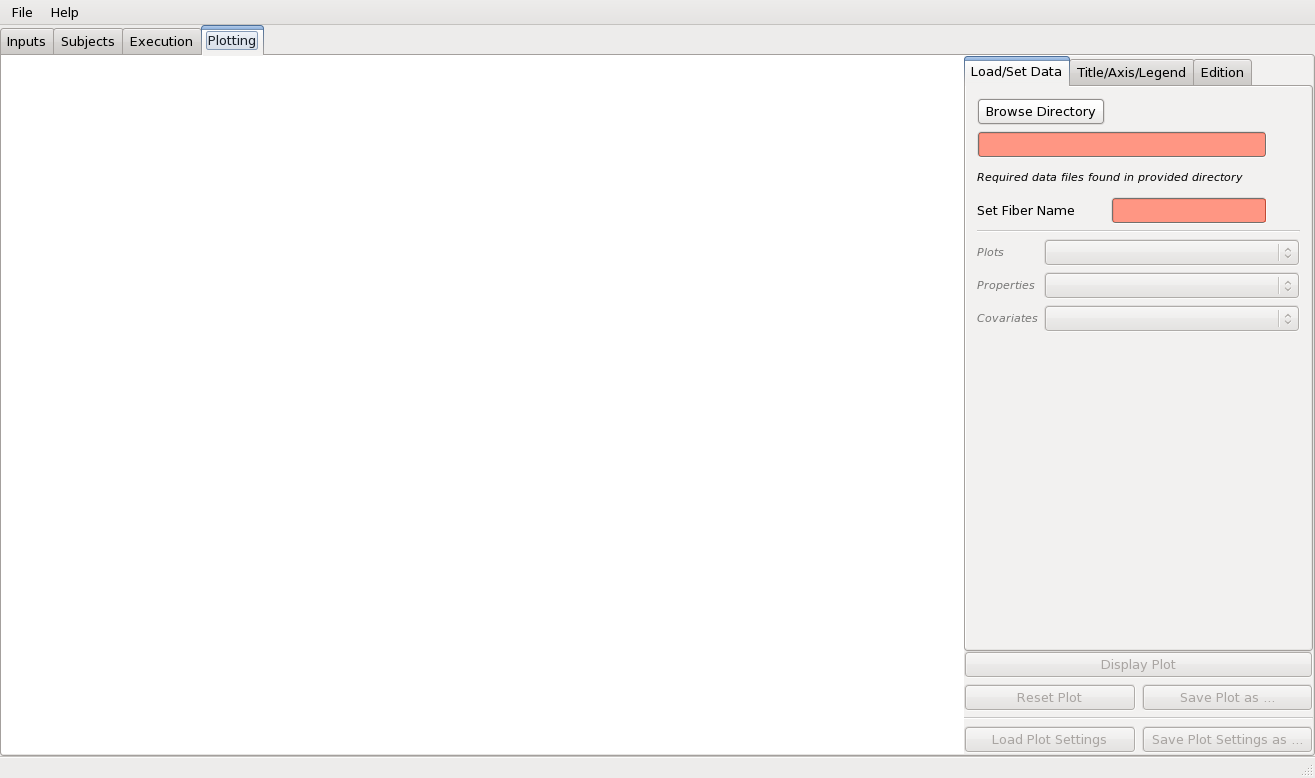
\includegraphics[width=1.0\textwidth]{plottingTab_Conf}
    	\caption{\textit{Para} settings (red)}
    	\label{fig:plottingTab_Conf}
    \end{figure}
	
	The configuration files are .json files. They have a very specific syntax. Templates for each configuration can be found \href{https://github.com/jeantm/FADTTSter/tree/master/doc/ConfigurationFiles_Example}{\underline{\textbf{here}}}.
	
	\subsection{Upload configurations to GUI}
	\begin{enumerate}
		\item Click on ``File''
		\item Select ``Load Parameters Configuration'' or ``Load Software Configuration'' depending on what you want to add
		\item Browse to the .json file containing the configuration wanted
		\item Select it
		\item Click on ``Open''
	\end{enumerate}
	\begin{figure}[!h]
		\centering
		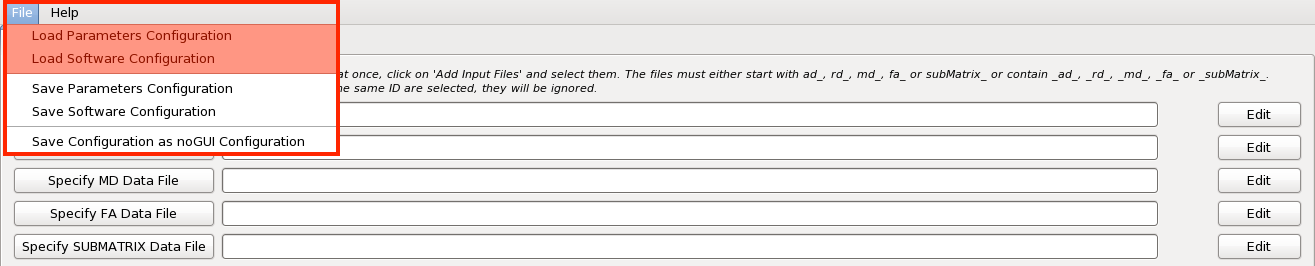
\includegraphics[width=1.0\textwidth]{configurationsLoad}
		\caption{Load configuration files and add them to the GUI}
		\label{fig:configurationsLoad}
	\end{figure}
	\vfill
    \newpage
    
	\subsection{Save configurations}
	\begin{enumerate}
		\item Click on ``File''
		\item Select ``Save Parameters Configuration'' or ``Save Software Configuration'' depending on what you want to save
		\item Browse to the folder where you want to keep the configuration
		\item Rename file if needed
		\item Click on ``Save''
	\end{enumerate}
	\begin{figure}[H]
		\centering
		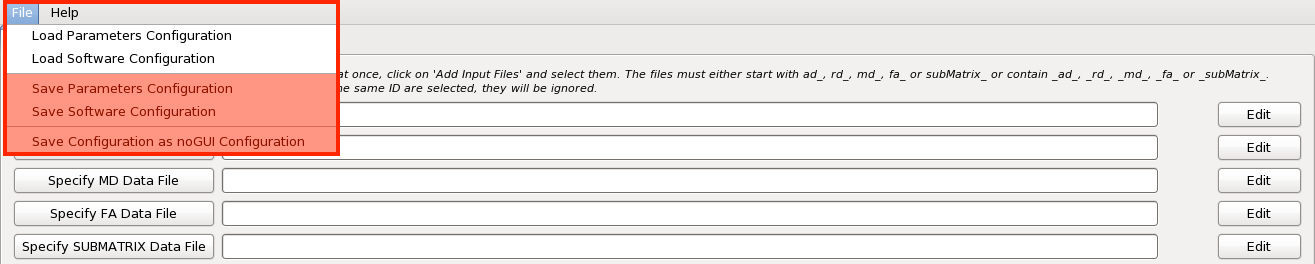
\includegraphics[width=1.0\textwidth]{configurationsSave}
		\caption{Save configurations}
		\label{fig:configurationsSave}
	\end{figure}
	\subparagraph{\textbf{Note:}} ``Save Configuration as noGUI Configuration'' saves the configuration in such a way that it can be used to run FADTTSter without the GUI.	
	\vfill
    \newpage
    
	\section{Plot settings}
	To help the user to work efficiently on the visualization of the results, the same system of .json files exits for the plot settings. All the settings value can be saved and uploaded in the GUI for the plotting tab.
	
	\subsection{Upload configurations to GUI}
	\begin{enumerate}
		\item Click on ``Load Plot Settings''
		\item Browse to the .json file containing the plot settings wanted
		\item Select it
		\item Click on ``Open''
	\end{enumerate}
	
	\subsection{Save configurations}
	\begin{enumerate}
		\item Click on ``Save Plot Settings as \ldots ''
		\item Browse to the folder where you want to save the settings
		\item Rename file if needed
		\item Click on ``Save''
	\end{enumerate}
	
	\begin{figure}[H]
		\centering
		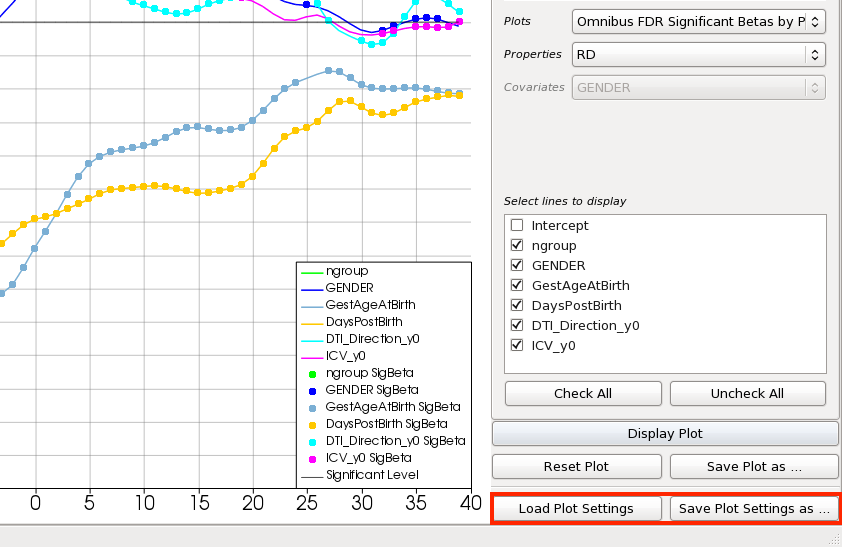
\includegraphics[width=1.0\textwidth]{loadSavePlotSettings}
		\caption{Load save plot settings}
		\label{fig:loadSavePlotSettings}
	\end{figure}
	\vfill
    \newpage
	
	\section{FADTTSter in command line}
	FADTTSter can be launched with some options before the GUI is only in the terminal. Here some examples illustrating how to use them:
	\begin{itemize}
		\item Launch FADTTSter within a GUI:
		\begin{lstlisting}[language=bash]
$ FADTTSter [-d] [--softConfig] [--paraConfig]
		\end{lstlisting}
		\textit{[-d]:} Path to a directory. When opening the GUI, a search will be made within the directory provided to find configation files. If files are found, they will automatically be loaded to the GUI. Files must be named as following: \textit{*para*.json} or \textit{*Para*.json}, \textit{*soft*.json} or \textit{*Soft*.json} and \textit{*noGUI*.json} or \textit{*NoGUI*.json}.\\
		\textit{[--softConfig]:} Path to the .json file containing the software configuration. The configuration will automatically be loaded to the GUI.\\
		\textit{[--paraConfig]:} Path to the .json file containing the parameters configuration. The configuration will automatically be loaded to the GUI.\\
		
		These parameters are independent of each other. However, if \textit{[-d]} and \textit{[--softConfig]} are use, the sofware configuration file provided by \textit{[--softConfig]} will take over the one found in the directory provided by \textit{[-d]}.
		
		\item Launch FADTTSter only using the terminal:
		\begin{lstlisting}[language=bash]
$ FADTTSter [--noGUI] [--noGUIConfig]
		\end{lstlisting}
		\textit{[--noGUI]:} Indicates that the GUI should not be displayed.\\
		\textit{[--noGUIConfig]:}  Path to the .json file containing the no-GUI configuration (parameters and software).\\
		
		FADTTSter will be run with the information provided in the no-GUI configuration file. \textit{[--noGUI]} and \textit{[--noGUIConfig]} MUST be run together! Otherwise, FADTTSter cannot be computed.
	\end{itemize}
\end{document}